\documentclass{article}
\usepackage{graphicx} % Required for inserting images

\usepackage{float}
\usepackage[preprint]{neurips_2024}

\usepackage[utf8]{inputenc} % allow utf-8 input
\usepackage[T1]{fontenc}    % use 8-bit T1 fonts
\usepackage{hyperref}       % hyperlinks
\usepackage{url}            % simple URL typesetting
\usepackage{booktabs}       % professional-quality tables
\usepackage{amsfonts}       % blackboard math symbols
\usepackage{nicefrac}       % compact symbols for 1/2, etc.
\usepackage{microtype}      % microtypography
\usepackage{xcolor}         % colors

\title{Figures and Data For: "Image Classification on Satellite Imagery For Sustainable Rainwater Harvesting Placement in Indigenous Communities of Northern Tanzania"}
\author{Roshan Taneja, Yuvraj Taneja}
\date{June 2024}

\begin{document}

\maketitle


\newpage

\begin{figure}[H]
    \centering
    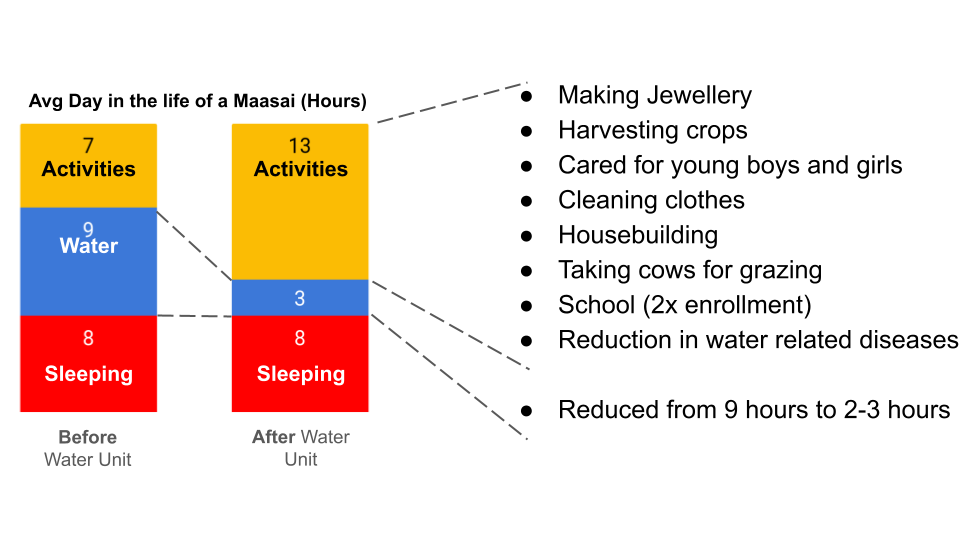
\includegraphics[width=1\linewidth]{images/beforeandafterwhu.png}
    \caption{Before and after the Water Harvesting Unit: Doubled the time spent on economic, social, and agricultural activities}
    \label{fig:bef_aft_results}
\end{figure}

\begin{figure}[H]
    \centering
    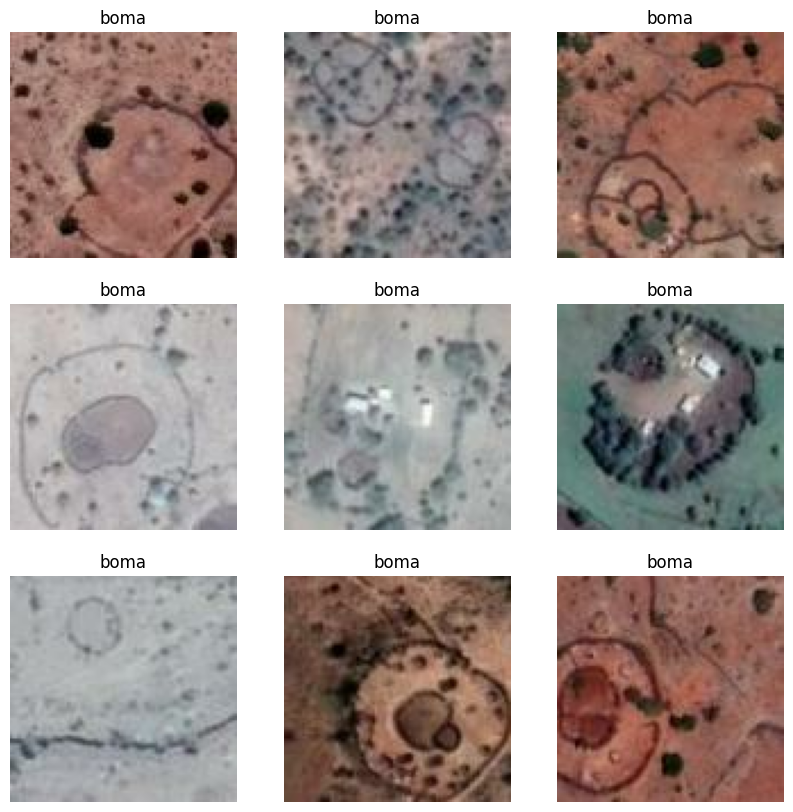
\includegraphics[width=0.8\linewidth]{images/types of bomas.png}
    \caption{Example of Variation in Landscape, Vegetation and Structure}
    \label{fig:types_of_bomas}
\end{figure}

\begin{figure}[H]
    \centering
    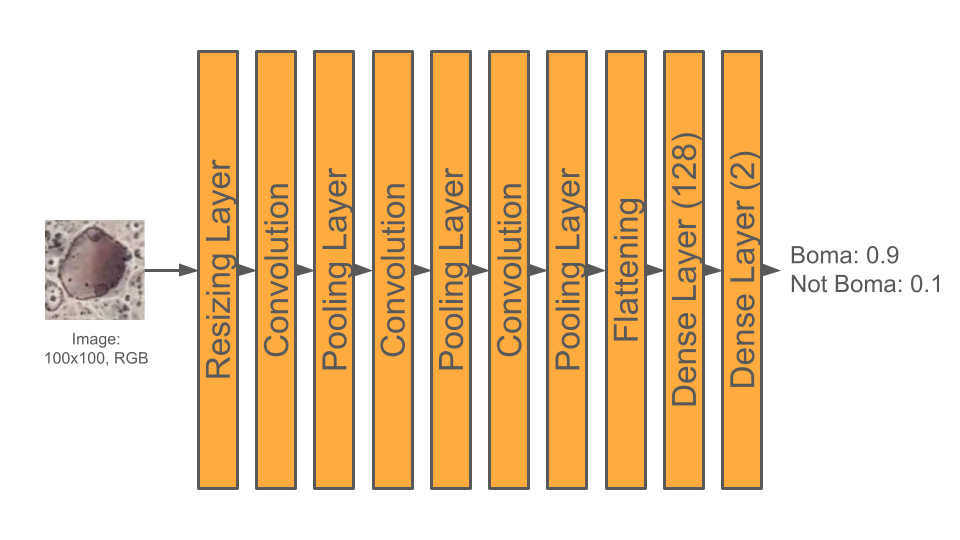
\includegraphics[width=1\linewidth]{images/Model Shape.png}
    \caption{Shape of the Model}
    \label{fig:model_shape}
\end{figure}

\begin{figure}[H]
    \centering
    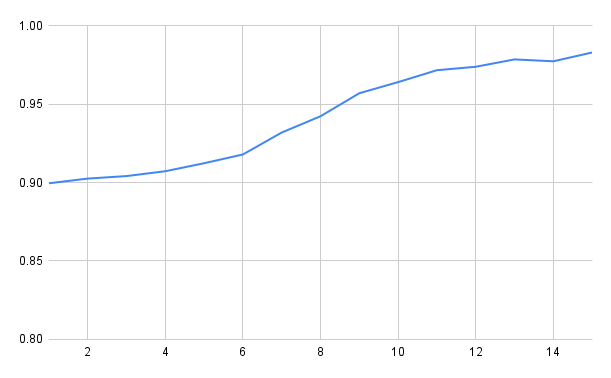
\includegraphics[width=1\linewidth]{images/Training Accuracy over 15 epochs.png}
    \caption{Training Accuracy over 15 epochs}
    \label{fig:Training_Accuracy}
\end{figure}

\begin{table}[H]
    \centering
    \begin{tabular}{rrrl}
    \multicolumn{1}{c}{\textbf{Epoch}} & \multicolumn{1}{c}{\textbf{Training Loss}} & \multicolumn{1}{c}{\textbf{Training Accuracy}} &  \\ \toprule
    1  & 0.3279 & 0.8995 &  \\
    2  & 0.3031 & 0.9025 &  \\
    3  & 0.2801 & 0.9041 &  \\
    4  & 0.2526 & 0.9072 &  \\
    5  & 0.2267 & 0.9123 &  \\
    6  & 0.1942 & 0.9179 &  \\
    7  & 0.1612 & 0.9319 &  \\
    8  & 0.1353 & 0.9423 &  \\
    9  & 0.1091 & 0.957  &  \\
    10 & 0.091  & 0.9641 &  \\
    11 & 0.075  & 0.9717 &  \\
    12 & 0.0653 & 0.9739 &  \\
    13 & 0.0543 & 0.9786 &  \\
    14 & 0.0546 & 0.9774 &  \\
    15 & 0.044  & 0.983  &  \\ \bottomrule
    \end{tabular}
    \caption{Raw data from Training for 15 epochs}
    \label{tab:training_raw_data}
\end{table}


\begin{figure}[H]
    \centering
    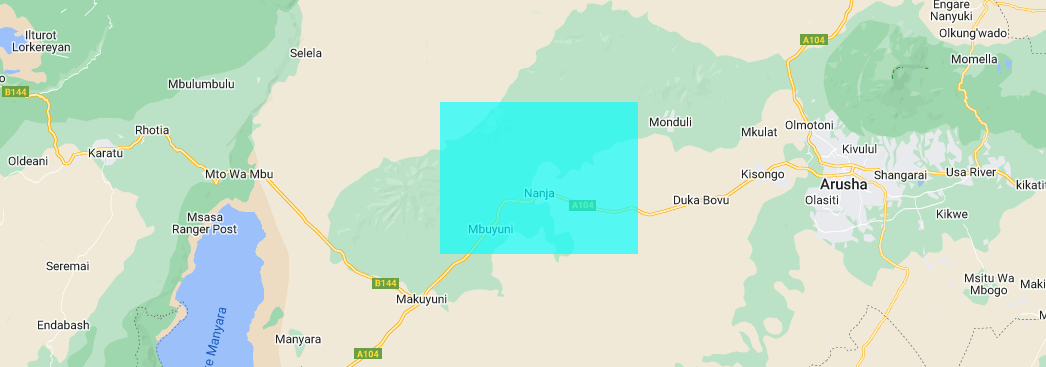
\includegraphics[width=1\linewidth]{images/studyarea.png}
    \caption{Designated Area for First Test, 260 square miles between Serengeti and Arusha}
    \label{fig:designated_area}
\end{figure}

\begin{figure}[H]
    \centering
    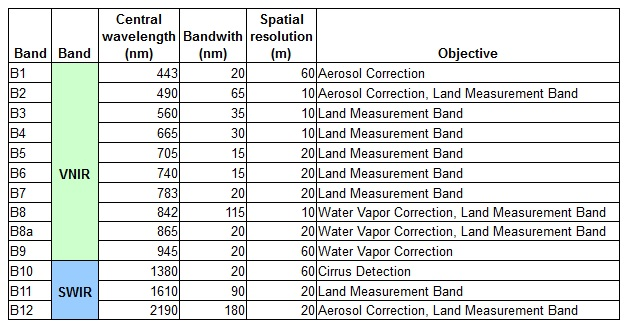
\includegraphics[width=1\linewidth]{images/copernicus_band_resolution.png}
    \caption{Band Resolutions Provided by Copernicus}
    \label{fig:cop_bands_chart}
\end{figure}

\begin{figure}[H]
    \centering
    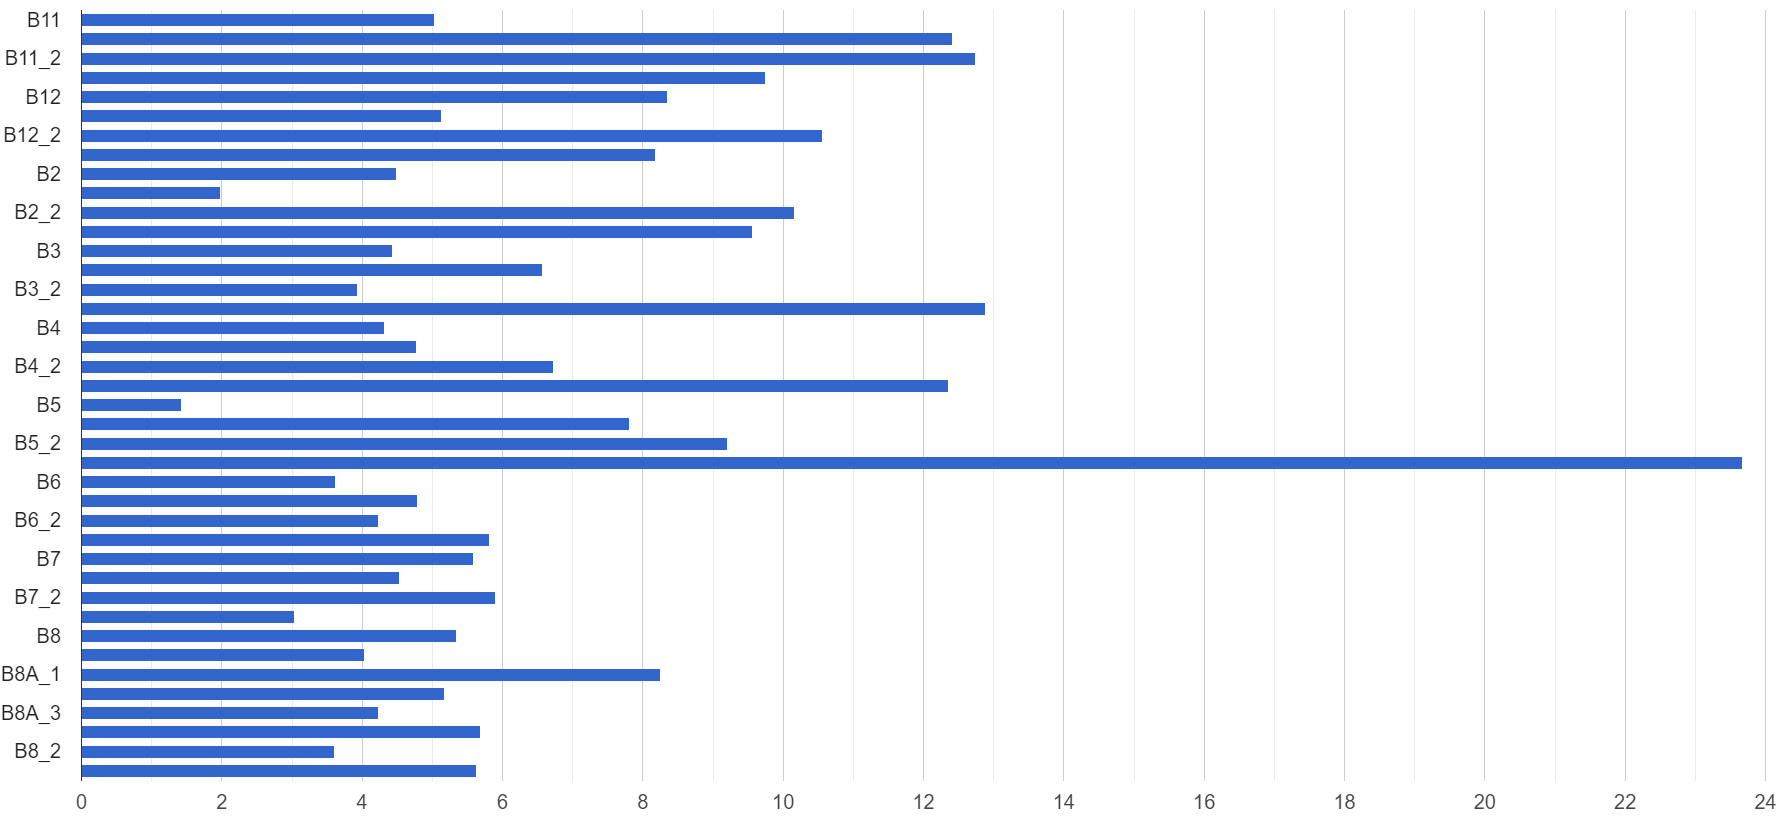
\includegraphics[width=1\linewidth]{images/bands importance.png}
    \caption{Variable Band Priority}
    \label{fig:band_importance}
\end{figure}

\begin{figure}[H]
\centering
    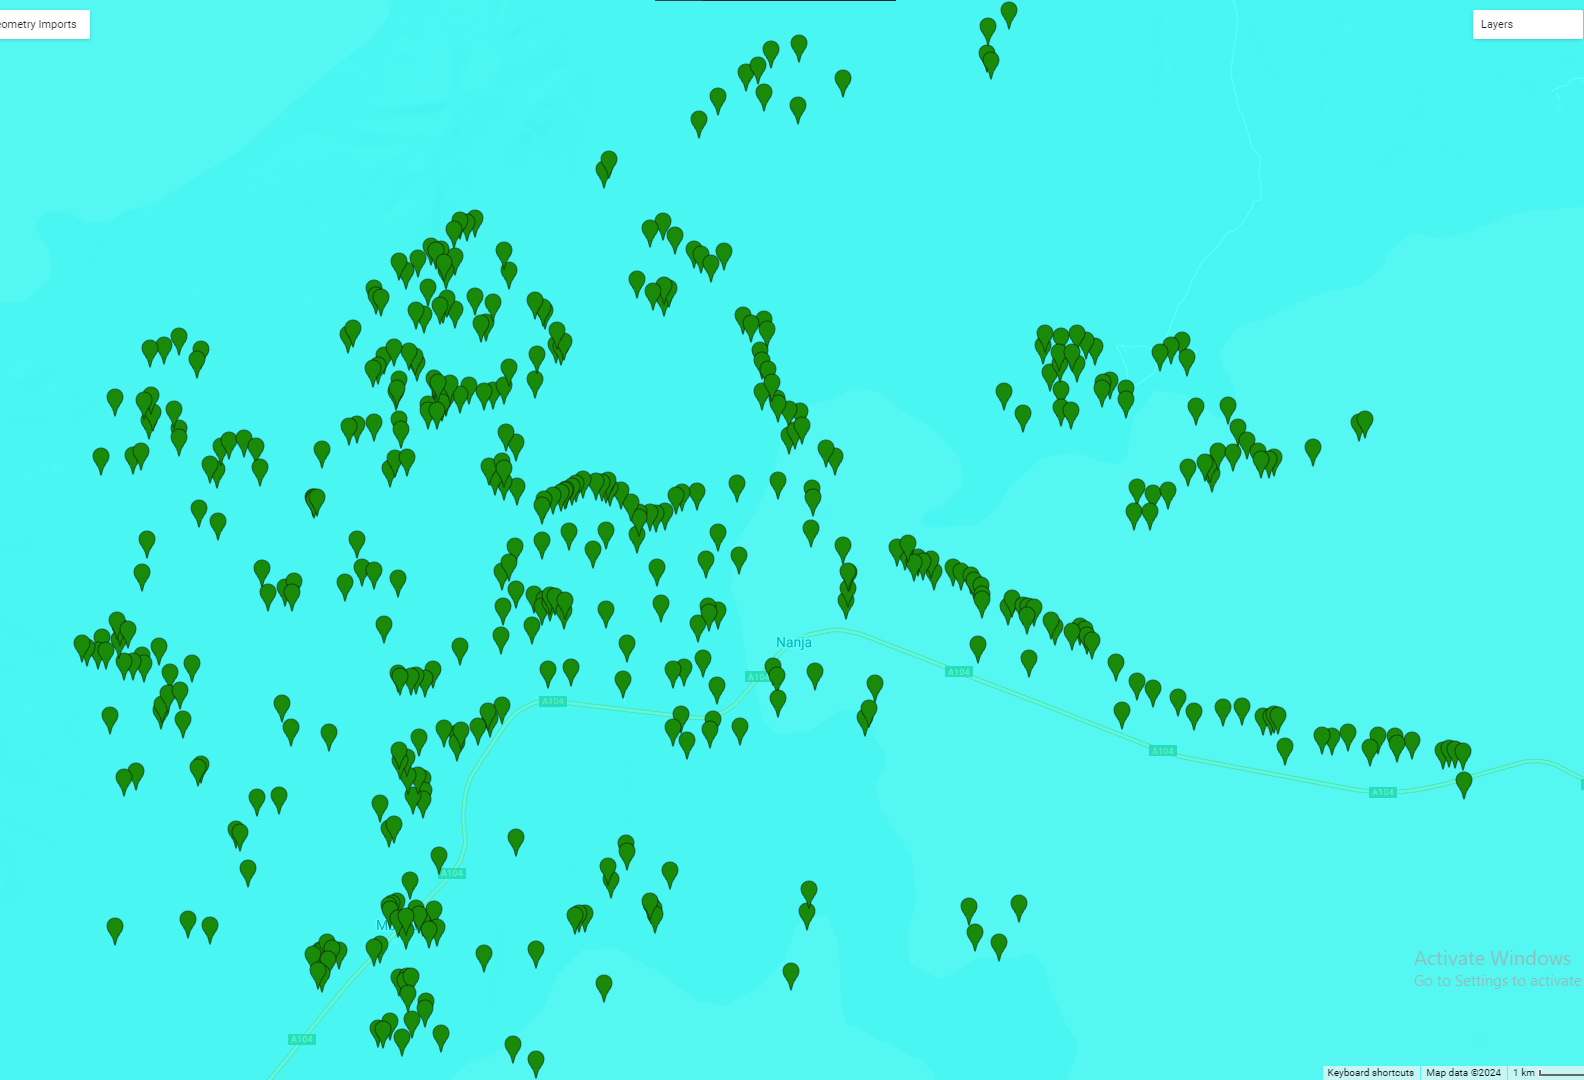
\includegraphics[width=1\linewidth]{images/cv_output.png}
    \caption{Output with relative coordinates}
    \label{fig:OutputOnSample}
\end{figure}

\begin{figure}[H]
    \centering
    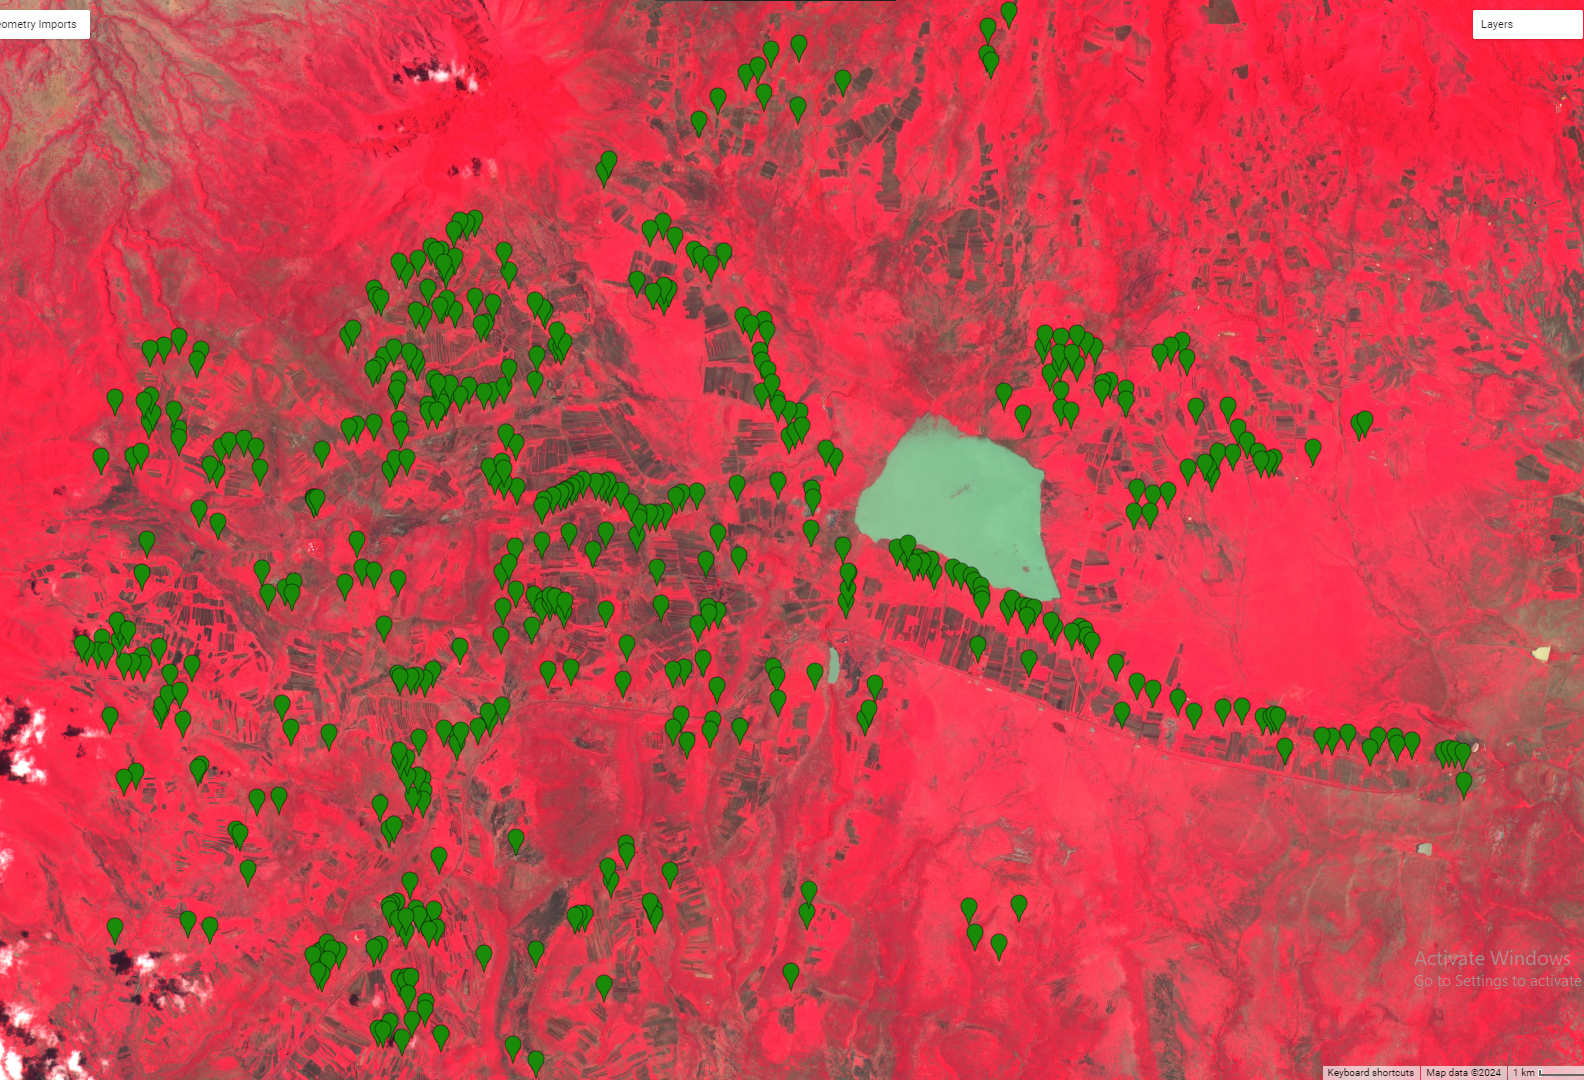
\includegraphics[width=1\linewidth]{images/Outputoverlayrealmap.png}
    \caption{Output Overlayed Over Image Stack}
    \label{fig:OverlayedMap}
\end{figure}

\begin{figure}[H]
    \centering
    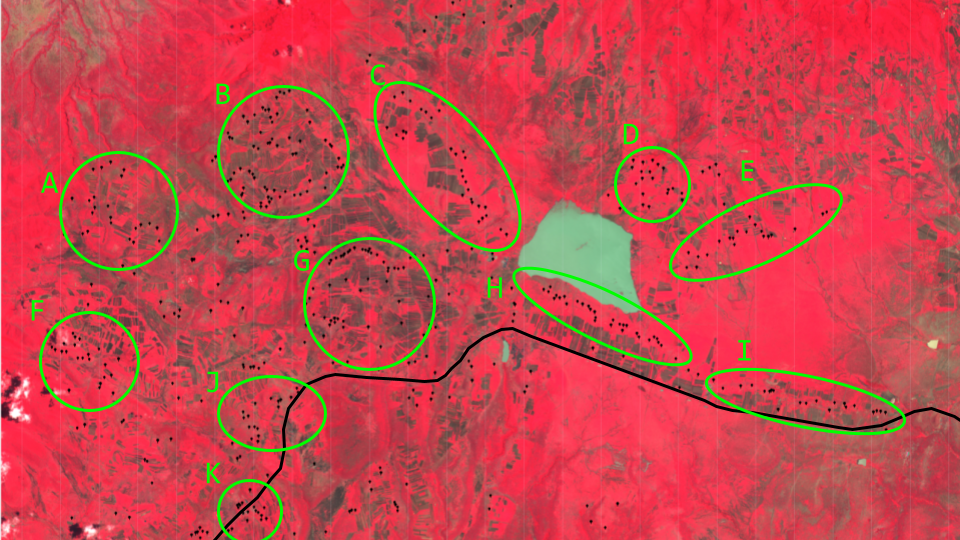
\includegraphics[width=1\linewidth]{images/Communities and Highway Highlighted.png}
    \caption{Large High-Density Community Collections of Bomas Highlighted with Major Highway}
    \label{fig:Communities and Major Highway}
\end{figure}

\begin{figure}[H]
    \centering
    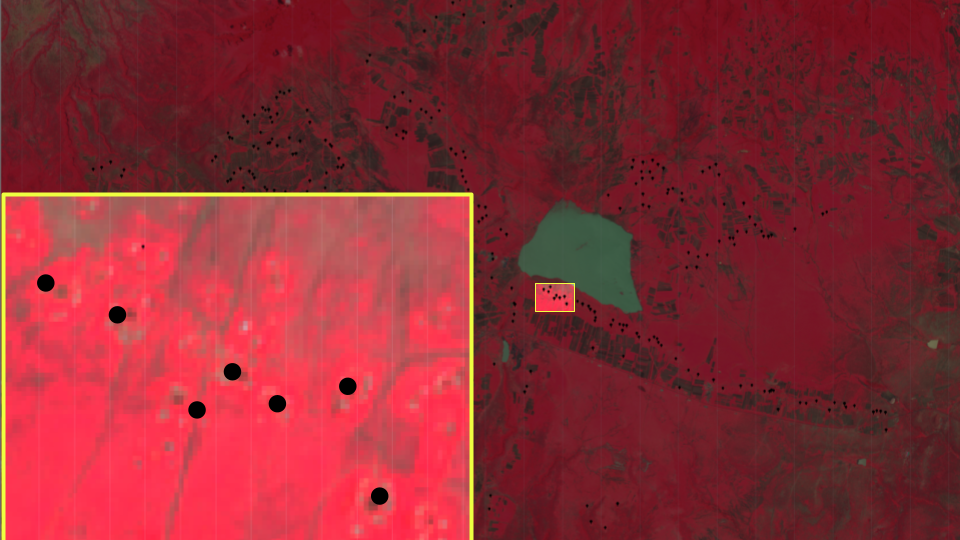
\includegraphics[width=1\linewidth]{images/zoomed in overlay.png}
    \caption{Zoomed In Portion on GEE}
    \label{fig:Zoomed_Overlayed}
\end{figure}

\begin{figure}[H]
    \centering
    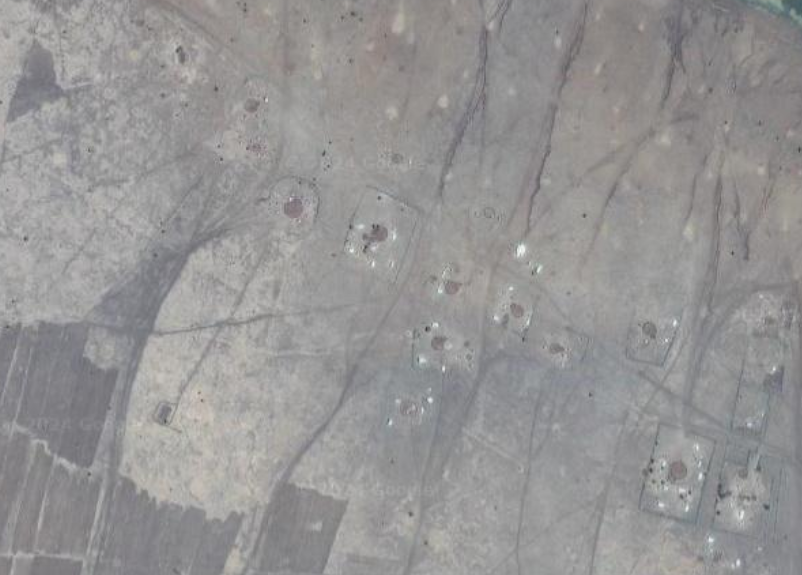
\includegraphics[width=1\linewidth]{images/zoomed google maps.png}
    \caption{Zoomed In Portion Displaying Exact same location with drone photography}
    \label{fig:enter-label}
\end{figure}

\begin{figure}[H]
    \centering
    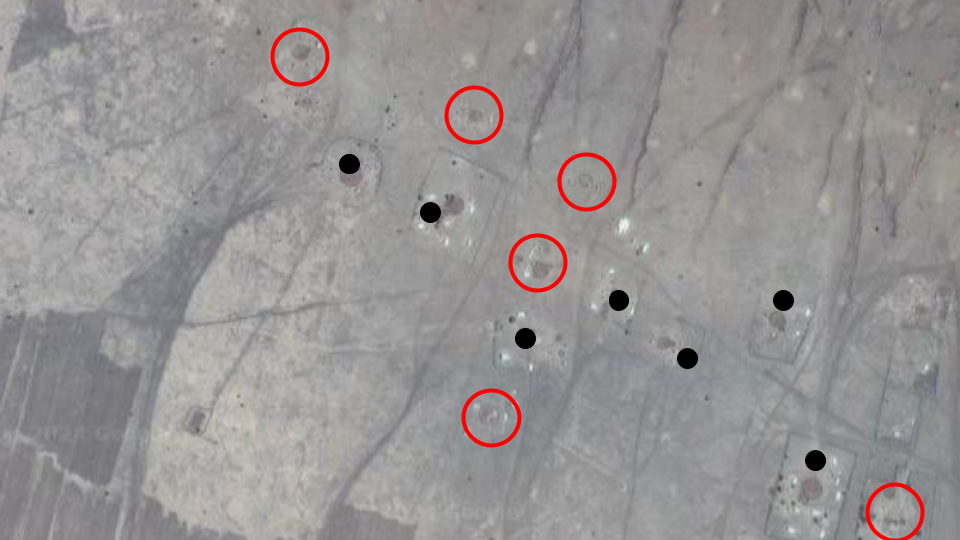
\includegraphics[width=1\linewidth]{images/zoomed google maps highlighted.png}
    \caption{Zoomed In Portion on Google Maps Displaying False Negatives}
    \label{fig:zoomed_google_maps}
\end{figure}

\end{document}